\chapter{Problema}\label{problema}

\section{Introducción}\label{problema:introduccion}

En algunas aplicaciones vinculadas a la clasificación, el objetivo final no es
determinar a qué clase (o clases) pertenece cada una de las instancias
individuales de un conjunto de datos no etiquetado, sino estimar la proporción
(tambíen llamada `prevalencia', `frecuencia relativa' o `probabilidad prior') de
cada clase en los datos sin etiquetar. En los últimos años se ha señalado que,
en estos casos, tiene sentido optimizar directamente algoritmos de aprendizaje
automático para este objetivo, en lugar de simplemente optimizar clasificadores
para etiquetar instancias individuales.

La tarea de ajustar estimadores de prevalencia de clases a través del
aprendizaje supervisado se conoce como `aprender a cuantificar' o, más
simplemente, cuantificar o {\it quantification\/} (término acuñado
por~\citet{forman2005counting}, quien planteó el problema por primera vez). Se
sabe que cuantificar mediante la clasificación de cada instancia sin etiquetar a
través de un clasificador estándar y luego contando las instancias que han sido
asignadas a cada clase (el método {\it Classify \& Count\/}) generalmente
conduce a estimadores de prevalencia de clases sesgados, es decir, obtienen poca
exactitud en la cuantificación. Como resultado, se han desarrollado métodos que
abordan la cuantificación como una tarea en sí.

Para ver la importancia de diferenciar el problema de cuantificación del de
clasificación, veamos dos ejemplos. En el primero, una empresa que ofrece un
servicio a sus clientes realiza una encuesta con varias preguntas para
determinar el grado de satisfacción de cada persona. El objetivo de le empresa
es determinar aquellos clientes que podrían no estar conformes con el servicio y
ofrecerles una mejora en las condiciones para retenerlos. En el segundo ejemplo,
una consultora analiza tweets para estimar el grado de aprobación de candidatos
políticos. Aquí, la consultora no está interesado en predecir si un individuo
específico está a favor o en contra, sino en cuántos encuestados, del número
total de encuestados, aprueban al candidato, es decir, en conocer la prevalencia
de la clase positiva.

Mientras en el primer escenario el interés es a nivel individual, en el último,
el nivel agregado es lo que importa; en otras palabras, en el primer escenario
la clasificación es el objetivo, mientras que en el segundo el verdadero
objetivo es la cuantificación. De hecho, en la mayoría de las aplicaciones las
predicciones que interesan no son a nivel individual sino a nivel colectivo;
ejemplos de tales campos son la investigación de mercado, la ciencia política,
las ciencias sociales, modelado ecológico y epidemiología.

\begin{figure}[h]
    \centering
    \begin{subfigure}[t]{0.4\textwidth}
        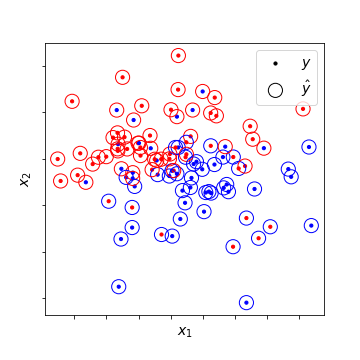
\includegraphics[width=\textwidth]{../plots_teoria/intro_scatterplot.png}
        \caption{Clasificación}
    \end{subfigure}
    \hfill
    \begin{subfigure}[t]{0.4\textwidth}
        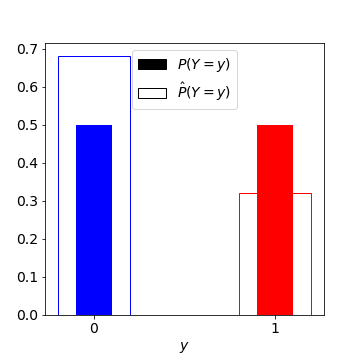
\includegraphics[width=\textwidth]{../plots_teoria/intro_barplot.png}
        \caption{Cuantificación}
    \end{subfigure}
    \caption{En la clasificación, la predicción es a nivel individual, mientras
    que en la cuantificación es a nivel agregado.}\label{fig:intro}
\end{figure}

En resumen, y generalizando no sólo para clasificación sino también a otros
problemas (regresión, ordinalidad, etc), la tarea de cuantificación consiste en
proporcionar predicciones agregadas para conjuntos de datos, en vez de
predicciones particulares sobre los datos individuales. Si bien en principio no
es necesario realizar predicciones por cada individuo, muchos de los métodos se
basan en obtener la cuantificación de esa manera, ya que hacer predicciones
individuales suele ser un requisito de por sí de las aplicaciones prácticas, o
porque ya existen en ellas modelos que las generen.

La literatura sobre métodos relacionados con cuantificación está un tanto
desconectada. Algunos de los métodos que pueden usarse como cuantificadores han
sido ideados para otros fines, principalmente para mejorar la precisión en
clasificación cuando cambia el dominio. El desempeño de este último grupo ha
sido normalmente estudiado solo en términos de mejora en las tareas de
clasificación pero no como cuantificadores. Dado este escenario, y debido a la
variedad de campos en los que ha surgido como una necesidad de aplicación, los
algoritmos que se pueden aplicar para tareas de cuantificación aparecen en
artículos que usan diferentes palabras clave y nombres, como {\it
counting\/}~\cite{lewis1995evaluating}, {\it prior probability
shift\/}~\cite{moreno2012unifying, storkey2009training}, {\it posterior
probability estimation\/}~\cite{alaiz2011class}, {\it class prior
estimation\/}~\cite{du2014class, chan2006estimating, zhang2010transfer}, {\it
class prior change\/}~\cite{du2014semi}, {\it prevalence
estimation\/}~\cite{barranquero2013study}, {\it class ratio
estimation\/}~\cite{asoh2012fast} o {\it class distribution
estimation\/}~\cite{gonzalez2013class, limsetto2011handling,
xue2009quantification}, por citar solo algunos de ellos.

\section{Tipos de Cuantificación}\label{problema:tipos}

Aunque el estudio de la cuantificación se ha centrado principalmente en el
dominio de clasificación, la cuantificación también aparece en otros tipos de
problemas de aprendizaje automático, como la regresión, la clasificación
ordinal, el aprendizaje sensible al costo y la cuantificación en redes.

De manera similar a la regresión, aprender a cuantificar admite diferentes
problemas de interés aplicativo, basados en cuántas clases distintas existen en
el problema, y en cuántas de las clases se pueden atribuir al mismo tiempo al
mismo individuo. Así, los problemas de cuantificación se dividen de esta manera:

\begin{enumerate}
    \item Etiquetado simple {\it (Single-Label Quantification -SLQ-)\/}: cuando
    cada individuo pertenece exactamente a una de las clases en
    $C=\{c_1,\dots,c_{\#C}\}$.
    \item Etiquetado múltiple {\it (Multi-Label Quantification -MLQ-)\/}: cuando
    cada individuo puede pertenecer a cualquier número de clases (cero, una o
    varias) en $C=\{c_1,\dots,c_{\#C}\}$.
    \item Cuantificación Binaria {\it (Binary Quantification -BQ-)\/}:
    \begin{enumerate}
        \item en {\it SLQ\/} con $\#C=2$, (en este caso $C=\{c_1,c_2\}$, y cada
        individuo pertenece a $c_1$ o $c_2$)
        \item en {\it MLQ\/} con $\#C=1$, (en este caso $C=\{c\}$, y cada
        individuo pertenece o no a $c$)
    \end{enumerate}
    \item Cuantificación Ordinal {\it (Ordinal Quantification -OQ-)\/}: cuando
    existe un orden $c_1 \prec \dots \prec c_{\#C}$ en
    $C=\{c_1,\dots,c_{\#C}\}$.
    \item Cuantificación de Regresión {\it (Regression Quantification -RQ-)\/}:
    cuando no hay un conjunto de clases involucradas, sino que cada individuo
    está etiquetado con una puntuación de valor real y la cuantificación
    equivale a estimar la fracción de ítems cuya puntuación está en un intervalo
    dado $[a, b]$ con ${a, b \in \mathbb{R}^d}$.
\end{enumerate}

\section{Marco teórico}\label{problema:marco_teorico}

Si hablamos entonces de cuantificación binaria, se tiene que por cada muestra $i
\in \{1,\dots,n\}$, $(\boldsymbol{X}_i,Y_i,S_i)$ es un vector de variables
aleatorias tal que $\boldsymbol{X}_i \in \mathbb{R}^d$ son las características
de la muestra, $Y_i \in C$ con $C=\{1,0\}$ indica la clase a la que pertenece y
$S_i \in \{1,0\}$ indica si fue etiquetada (y pertenece entonces al conjunto de
entrenamiento) o no. Es decir, cuando $S_i=0$, entonces $Y_i$ no es observable.
El objectivo es estimar $\theta:= \mathbb{P}(Y=1|S=0)$\footnote{En
cuantificación, se lo nombra generalmente como $p$ (o $p_1,\dots,p_{\#C}$ o
$p(c)$ para el caso multiclase) en vez de $\theta$, por lo que en este trabajo
también se usará esta nomenclatura.}, es decir, la prevalencia de etiquetas
positivas entre muestras no etiquetadas. Esta prevalencia no se asume de ser la
misma que en las muestras etiquetadas, $\mathbb{P}(Y=1|S=1)$. Además, el
estimador de $\theta$ debe depender sólo de los datos disponibles, es decir, de
las características de todas las muestras y de las etiquetas que fueron
obtenidas. Los supuestos que se asumen~\cite{vaz2019quantification} son:

\begin{itemize}
  \item $(\boldsymbol{X}_1,Y_1,S_1) \dots (\boldsymbol{X}_n,Y_n,S_n)$ son
  independientes
  \item Por cada $s \in \{0,1\}$,
  $(\boldsymbol{X}_1,Y_1)|S_1=s,\dots,(\boldsymbol{X}_n,Y_n)|S_n=s$ son
  idénticamente distribuidas.
  \item Por cada $(y_1,\dots,y_n)\in{\{0,1\}}^n$,
  $(\boldsymbol{X}_1,\dots,\boldsymbol{X}_n)$ es independiente de
  $(S_1,\dots,S_n)$ condicionado a $(Y_1,\dots,Y_n)=(y_1,\dots,y_n)$
\end{itemize}

Usando la distribución de probabilidad conjunta, podemos factorizar usando las
distribuciones condicionales:
\begin{equation}
    \mathbb{P}(\boldsymbol{X},Y,S)=\mathbb{P}(\boldsymbol{X}|Y,S)\mathbb{P}(Y|S)\mathbb{P}(S)
\end{equation}
Luego, usando el tercer supuesto mencionado, podemos
hacer~\cite{moreno2012unifying}:
\begin{equation}
    \mathbb{P}(\boldsymbol{X},Y,S)=\mathbb{P}(\boldsymbol{X}|Y)\mathbb{P}(Y|S)\mathbb{P}(S)
\end{equation}
Si bien existen varios métodos propuestos para el aprendizaje de
cuantificación~\cite{esuli2023learning, gonzalez2017review}, el mismo es todavía
relativamente desconocido incluso para expertos en aprendizaje automático. La
razón principal es la creencia errónea de que es una tarea trivial que se puede
resolver usando un método directo, como {\it CC}. La cuantificación requiere
métodos más sofisticados si el objetivo es obtener modelos óptimos, y su
principal dificultad radica en la definición del problema, ya que las
distribuciones de los datos de entrenamiento y de prueba pueden ser distintas.
Por ejemplo, si la diferencia entre $\mathbb{P}(Y=1|S=0)$ y
$\mathbb{P}(Y=1|S=1)$ es grande, los métodos simples como {\it CC\/} suelen
tener bajo rendimiento.


\section{Cambios en las distribuciones de los datos}\label{problema:cambios}

En lo últimos años ha habido un interés creciente en las aplicaciones que
presentan cambios en las distribuciones de datos (conocido en la blibliografía
por su término en inglés {\it dataset shift\/}). Estos problemas comparten el
hecho de que la distribución de los datos utilizados para entrenar es diferente
a la de los datos que se usan para predecir. Al igual que para el área de la
cuantificación, aquí también la literatura sobre el tema está dispersa y
diferentes autores usan diferentes nombres para referirse a los mismos
conceptos, o usan el mismo nombre para diferentes conceptos.

Teniendo en cuenta que en los problemas de clasificación tenemos:

\begin{itemize}
    \item Un conjunto de características o covariables $\boldsymbol{X}$.
    \item Una variable de respuesta $Y$.
    \item Una distribución de probabilidad conjunta
    $\mathbb{P}(Y=y,\boldsymbol{X=x})$.
\end{itemize}

La probabilidad conjunta $\mathbb{P}(Y,\boldsymbol{X})$ luego se puede escribir
como $\mathbb{P}(Y|\boldsymbol{X})\mathbb{P}(\boldsymbol{X})$ o como
$\mathbb{P}(\boldsymbol{X}|Y)\mathbb{P}(Y)$. Por otro lado, cuando usamos los
términos de entrenamiento ({\it train\/}) y prueba ({\it test\/}), nos referimos
a las datos disponibles para entrenar al clasificador y los datos presentes en
el entorno en el que se implementará el clasificador, respectivamente. Podemos
entonces también separar los datos en dos distribuciones distintas,
condicionando a la vaiable $S$ definida en~\ref{problema:marco_teorico}, siendo
$\mathbb{P}_{tr}(Y,\boldsymbol{X})=\mathbb{P}(Y,\boldsymbol{X}|S=1)$ y
$\mathbb{P}_{tst}(Y,\boldsymbol{X})=\mathbb{P}(Y,\boldsymbol{X}|S=0)$.

El {\it dataset shift\/} aparece cuando las distribuciones conjuntas de
entrenamiento y de prueba son diferentes, es decir, cuando
$\mathbb{P}_{tr}(Y,\boldsymbol{X}) \neq
\mathbb{P}_{tst}(Y,\boldsymbol{X})$.~\citet{moreno2012unifying} distingue las
distintas variantes del dataset shift según qué elementos mencionados
anteriormente cambian:

\begin{itemize}
    \item {\it Covariate shift}, cuando $\mathbb{P}_{tr}(Y|\boldsymbol{X}) =
    \mathbb{P}_{tst}(Y|\boldsymbol{X})$ y $\mathbb{P}_{tr}(\boldsymbol{X}) \neq
    \mathbb{P}_{tst}(\boldsymbol{X})$
    \item {\it Prior probability shift}, cuando
    $\mathbb{P}_{tr}(\boldsymbol{X}|Y) = \mathbb{P}_{tst}(\boldsymbol{X}|Y)$ y
    $\mathbb{P}_{tr}(Y) \neq \mathbb{P}_{tst}(Y)$
    \item {\it Concept shift}, cuando $\mathbb{P}_{tr}(Y|\boldsymbol{X}) \neq
    \mathbb{P}_{tst}(Y|\boldsymbol{X})$ y $\mathbb{P}_{tr}(\boldsymbol{X}) =
    \mathbb{P}_{tst}(\boldsymbol{X})$ o $\mathbb{P}_{tr}(\boldsymbol{X}|Y) \neq
    \mathbb{P}_{tst}(\boldsymbol{X}|Y)$ y $\mathbb{P}_{tr}(Y) =
    \mathbb{P}_{tst}(Y)$
\end{itemize}

Otros tipos de dataset shift surgen cuando $\mathbb{P}_{tr}(Y|\boldsymbol{X})
\neq \mathbb{P}_{tst}(Y|\boldsymbol{X})$ y $\mathbb{P}_{tr}(\boldsymbol{X}) \neq
\mathbb{P}_{tst}(\boldsymbol{X})$ y cuando $\mathbb{P}_{tr}(\boldsymbol{X}|Y)
\neq \mathbb{P}_{tst}(\boldsymbol{X}|Y)$ y $\mathbb{P}_{tr}(Y) \neq
\mathbb{P}_{tst}(Y)$. Sin embargo, estos tipos de cambios no se consideran
generalmente en la literatura ya que aparecen mucho más raramente, o incluso
porque son dificiles o imposibles de resolver.

Está claro que el problema de cuantificación se trata de un caso donde
$\mathbb{P}_{tst}(Y)$ es desconocido. Además, la mayoría de los métodos de
cuantificación propuestos asumen que $\mathbb{P}_{tr}(\boldsymbol{X}|Y) =
\mathbb{P}_{tst}(\boldsymbol{X}|Y)$, por lo que estarían dentro de los casos de
{\it prior probability shift}.

Por otro lado, en la mayoría de los casos el objetivo final de la implementación
es estimar algún parámetro de $\mathbb{P}_{tst}(Y)$. Por ejemplo, como ya
mencionamos anteriormente, en la cuantificación binaria, se desea estimar
$\theta:= \mathbb{P}(Y=1|S=0)$, o lo que es lo mismo, $p_{tst}:=
\mathbb{P}_{tst}(Y=1)$. Es decir, en la cuantificación la tarea indirectamente
suele ser aprender a aproximar una distribución desconocida (observando sólo
características de una muestra) mediante una distribución conocida. En
consecuencia, prácticamente todas las medidas de evaluación para la
cuantificación son divergencias, es decir, medidas de cómo una distribución
pronosticada difiere de la distribución real.

\begin{figure}[h]
    \centering
    \begin{subfigure}[t]{0.4\textwidth}
        \centering
        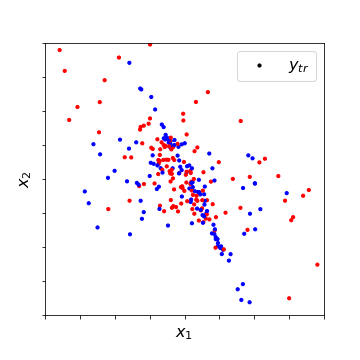
\includegraphics[width=\textwidth]{../plots_teoria/cambios_train_scatterplot.png}
        \caption{Muestra de entrenamiento}\label{cambios:datos_tr}
    \end{subfigure}
    \hfill
    \begin{subfigure}[t]{0.4\textwidth}
        \centering
        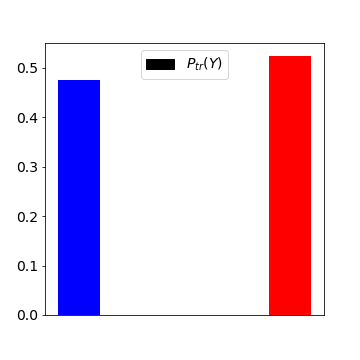
\includegraphics[width=\textwidth]{../plots_teoria/cambios_train_barplot.png}
        \caption{Prevalencia de clases en muestra de
        entrenamiento}\label{cambios:prevalencia_tr}
    \end{subfigure}
    \medskip
    \begin{subfigure}[t]{0.4\textwidth}
        \centering
        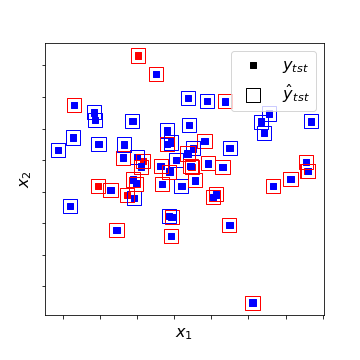
\includegraphics[width=\textwidth]{../plots_teoria/cambios_test_scatterplot.png}
        \caption{Clasificación en muestra de prueba. Para el modelo, las
        $y_{tst}$ son desconocidas.}\label{cambios:clasificacion_tst}
    \end{subfigure}
    \hfill
    \begin{subfigure}[t]{0.4\textwidth}
        \centering
        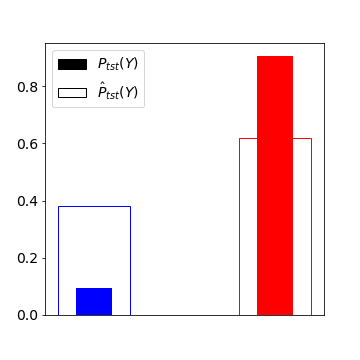
\includegraphics[width=\textwidth]{../plots_teoria/cambios_test_barplot.png}
        \caption{Prevalencia de clases verdadera y cuantificación en muestra de
        prueba}\label{cambios:cuantificacion_tst}
    \end{subfigure}
    \caption{El {\it prior probability shift\/} propio de los problemas de
    cuantificación puede hacer que los métodos simples de cuantificación, como
    {\it CC}, tengan grandes errores.}\label{fig:cambios}
\end{figure}

\section{El problema de clasificar y contar}\label{problema:clasificar_y_contar}

En ausencia de métodos para estimar los valores de prevalencia de clase de forma
directa, el primer método que suele pensarse para hacerlo es {\it Classify \&
Count}, es decir, clasificar cada individuo sin etiquetar y estimar los valores
de prevalencia de clase contando los individuos que fueron asignados a cada
clase. Sin embargo, esta estrategia es subóptima: si bien un clasificador
perfecto es también un cuantificador perfecto, un buen clasificador puede ser un
mal cuantificador. Para ver esto, se puede ver la definición de $F_1$, una
función de evaluación estándar para la clasificación binaria, que se define
como:
\begin{equation}
    F_1 = \frac{2 \cdot tp}{2 \cdot tp + fp + fn}
\end{equation}
donde $tp$, $fp$, $fn$ indican el número de verdaderos positivos, falsos
positivos y falsos negativos, respectivamente. Un buen clasificador puede ser un
mal cuantificador ya que $F_1$ considera buenos aquellos clasificadores que
mantienen la suma $fp + fn$ al mínimo; sin embargo, el objetivo de un algoritmo
de cuantificación debe ser mantener al mínimo $|fp-fn|$.

El análisis teórico de esta cuestión se basa en el supuesto de {\it prior
probability shift\/}~\ref{problema:cambios}. Bajo tal supuesto, la estimación
$\hat p$ obtenida por el enfoque {\it CC\/} depende sólo de las características
del clasificador, definido (para el caso binario) por su tasa de verdaderos
positivos ($tpr$), su tasa de falsos positivos ($fpr$) y de la prevalencia real
($p$):
\begin{equation}\label{ecuacion:tpr_fpr}
    \hat p(p) = p \cdot {tpr} + (1-p) \cdot {fpr}
\end{equation}
\begin{figure}[h]
    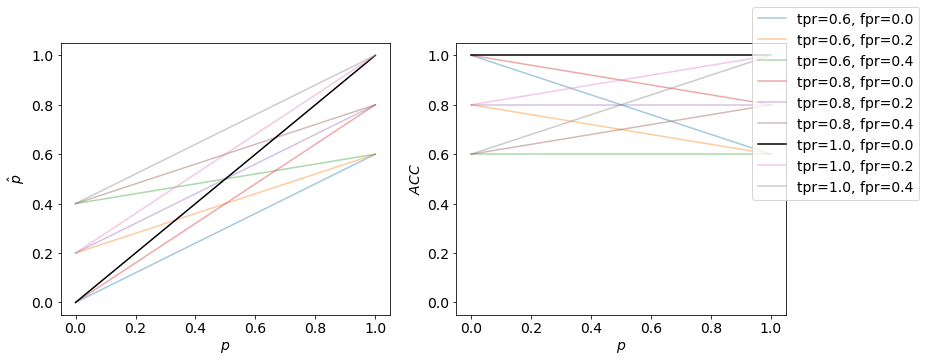
\includegraphics[width=\textwidth]{../plots_teoria/cc_tpr_fpr.png}
    \caption{La línea negra representa el cuantificador y clasificador perfecto,
    respectivamente. Las otras líneas muestran las estimaciones teóricas de
    $\hat p$ resultantes de aplicar la ecuación~\ref{ecuacion:tpr_fpr}, y el
    {\it accuracy\/} correspondiente al clasificador, según se varían los
    valores de $tpr$ y $fpr$}\label{fig:cc_tpr_fpr}
\end{figure}

El mal desempeño de {\it CC\/} fue demostrado mediante el siguiente teorema
por~\citeauthor{forman2008quantifying}:

\begin{theorem}[Toerema de Forman]
    \citep[p.169]{forman2008quantifying}\label{teorema:forman} Para un
    clasificador imperfecto, el método {\it CC\/} subestimará la porporción
    verdadera de ejemplos positivos $p$ en un conjunto de prueba para $p>p^*$, y
    sobreestimará para $p<p^*$, donde $p^*$ es la proporción particular en la
    cual el método {\it CC\/} estima de forma correcta. Es decir, el método {\it
    CC\/} estima exactamente $p^*$ para un conjunto de prueba con $p^*$ muestras
    positivas.
\end{theorem}

La demostración (ver todos los detalles en~\citep[p.170]{forman2008quantifying})
supone que el cuantificador {\it CC\/} produce una predicción perfecta para una
prevalencia concreta, llamada $p^*$, y estudia su comportamiento cuando la
prevalencia cambia ligeramente. Suponiendo que $\hat p(p^*) = p^*$, cuando la
prevalencia cambia en una cantidad $\Delta \neq 0, p^* + \Delta$, la estimación
del método CC en tal caso será:
\begin{align}
\begin{split}
    \hat p(p^* + \Delta) &= (p^* + \Delta) \cdot {tpr} + (1-(p^* + \Delta)) \cdot {fpr} \\
    &= \hat p(p^*) + ({tpr} - {fpr}) \cdot \Delta \\
    &= p^* + ({tpr} - {fpr}) \cdot \Delta
\end{split}
\end{align}
La predicción del método {\it CC\/} será perfecta, $\hat p(p^* + \Delta) = (p^*
+ \Delta)$, sólo cuando el clasificador también es perfecto (${tpr} = 1$, ${fpr}
= 0$ y por tanto ${tpr} - {fpr} = 1$). Pero en el caso habitual, en el cual el
clasificador es imperfecto ($0 \leq {tpr} - \text {fpr} < 1$), cuando la
prevalencia aumenta ($\Delta > 0$), {\it CC\/} la subestima ($\hat p < p^* +
\Delta $), y cuando la prevalencia disminuye ($\Delta < 0$), {\it CC\/} la
sobreestima ($\hat p > p^* + \Delta $).

Un buen clasificador puede estar sesgado, es decir, puede mantener sus falsos
positivos al mínimo sólo a expensas de una cantidad sustancialmente mayor de
falsos negativos (o viceversa); si este es el caso, el clasificador es un mal
cuantificador. Este fenómeno no es infrecuente, especialmente en presencia de
datos desbalanceados. En tales casos, los algoritmos que minimizan las funciones
de pérdida de clasificacion ({\it Hamming}, {\it hinge}, etc) suelen generar
clasificadores con tendencia a elegir la clase mayoritaria, lo que implica un
número mucho mayor de falsos positivos que de falsos negativos para la clase
mayoritaria, lo que significa a su vez que tal algoritmo tenderá a subestimar
las clases minoritarias.

Los argumentos anteriores indican que no se debe considerar la cuantificación
como un mero subproducto de la clasificación, y debe estudiarse y resolverse
como una tarea en sí misma. Hay al menos otros dos argumentos que apoyan esta
idea. Uno es que las funciones que se utilizan para evaluar la clasificación no
se pueden utilizar para evaluar la cuantificación, ya que estas funciones miden,
en general, cuántos individuos han sido mal clasificados, y no cuánto difiere la
prevalencia de clase estimada del valor real. Esto significa que los algoritmos
que minimizan estas funciones están optimizados para la clasificación, y no para
la cuantificación. Un segundo argumento presentado por
~\citet{forman2008quantifying} es que los métodos diseñados específicamente para
cuantificar requieren menos datos de entrenamiento para alcanzar la misma
precisión de cuantificación que los métodos estándar basados en {\it CC}. Si
bien esta observación es de naturaleza empírica, también existen argumentos
teóricos que sustentan este hecho~\cite{vapnik1999overview}.

\section{Cuantificadores para la mejora de la
Clasificación}\label{problema:mejora}

Debido a los problemas mencionados anteriormente de los clasificadores frente a
cambios en las distribuciones de los datos y frente a datos desbalanceados, los
algoritmos de cuantificación están cada vez más frecuentemente también siendo
usados en tareas que requieren predicciones individuales. Los mismos se emplean
como suplemento de clasificadores para suplir sus defectos frente a estos
problemas, ya que en algunos casos no sólo predicen los valores agregados, sino
que también mejoran las predicciones a nivel individual.

Por ejemplo, el {\it prior probability shift\/} puede hacer que los
clasificadores performen de manera subóptima. En el caso del clasificador óptimo
de Bayes, dado por:
\begin{equation}\label{ecuacion:bayes}
    h(\boldsymbol{x}) = \argmax_{y} p_{Y|\boldsymbol{X}=\boldsymbol{x}}(y) = \argmax_{y} \frac{p_{\boldsymbol{X}|Y=y}(\boldsymbol{x})p_Y(y)}{p_{\boldsymbol{X}}(\boldsymbol{x})}
\end{equation}
la decisión del clasificador depende de $p_Y(y)$, que es estimado con el dataset
de entrenamiento, siendo $\hat p_Y(y=1) = p_{tr}$. Es decir, que en caso de
$\mathbb{P}_{tr}(Y) \neq \mathbb{P}_{tst}(Y)$, la decisión final del
clasificador puede verse afectada negativamente. Para mejorar el rendimiento del
clasificador frente a estos casos, se debería usar $\hat p_Y(y=1) = p_{tst}$,
pero como $p_{tst}$ es generalmente desconocido, se puede usar un método de
cuantificación para estimarlo~\cite{saerens2002adjusting, alaiz2011class,
zhang2010transfer, xue2009quantification}.

Los métodos de cuantificación pueden usarse no sólo para mejorar el rendimiento
general de un clasificador, sino también para mejorar su equidad o {\it
fairness\/}~\cite{biswas2021ensuring}, es decir, su posibilidad de predecir
resultados independientes de un cierto conjunto de variables que consideramos
sensibles y no relacionadas con él (e.j.:~género, etnia, orientación sexual,
etc.). Por ejemplo, suponiendo que una variable $S$ debe considerarse sensible,
se puede estimar $\mathbb{P}_{tr}(Y|S)$. Luego, si los datos de entrenamiento
están sesgados, por ejemplo, con $\mathbb{P}_{tr}(Y=1|S=1) \gg
\mathbb{P}_{tr}(Y=1|S=0)$, pero se sabe que en las muestras a inferir esto no es
así, se puede optimizar el modelo de clasificación imponiento alguna penalidad
basada en la estimación de $\mathbb{P}_{tst}(Y|S)$, siendo esta última obtenido
por un cuantificador.
